%% 
%% ACS project dissertation template. 
%% 
%% Currently designed for printing two-sided, but if you prefer to 
%% print single-sided just remove ",twoside,openright" from the 
%% \documentclass[] line below. 
%%
%%
%%   SMH, May 2010. 


\documentclass[a4paper,12pt,twoside,openright]{report}


%%
%% EDIT THE BELOW TO CUSTOMIZE
%%

\def\authorname{David Brazdil\xspace}
\def\authorcollege{Trinity Hall\xspace}
%\def\authoremail{Sarah.Jones@cl.cam.ac.uk}
\def\dissertationtitle{Qishr: Capability-based Protection for the Java Native Interface}
\def\wordcount{14,235}


\usepackage{epsfig,graphicx,parskip,setspace,tabularx,xspace,url,listings,color,paralist,microtype,lipsum}

\newcommand{\reg}[1]{\texttt{\$#1}}
\newcommand{\insn}[1]{\texttt{#1}}
\newcommand{\keyword}[1]{\textsf{#1}}
\newcommand{\class}[1]{\texttt{#1}}
\newcommand{\tool}[1]{\emph{#1}}
\newcommand{\lib}[1]{\tool{lib#1}}


%% START OF DOCUMENT
\begin{document}

\lstset{
	basicstyle=\tt\footnotesize,	% the size of the fonts that are used for the code
	numbers=left,			% where to put the line-numbers
	numberstyle=\footnotesize,	% the size of the fonts that are used for the line-numbers
	stepnumber=1,			% the step between two line-numbers. If it is 1 each line will be numbered
	numbersep=5pt,			% how far the line-numbers are from the code
	backgroundcolor=\color{white},	% choose the background color. You must add \usepackage{color}
	showspaces=false,		% show spaces adding particular underscores
	showstringspaces=false,		% underline spaces within strings
	showtabs=false,			% show tabs within strings adding particular underscores
	frame=leftline,			% adds a frame around the code
	tabsize=2,			% sets default tabsize to 2 spaces
	captionpos=b,			% sets the caption-position to bottom
	breaklines=true,		% sets automatic line breaking
	breakatwhitespace=false,	% sets if automatic breaks should only happen at whitespace
	escapeinside={\%*}{*)},		% if you want to add a comment within your code
	captionpos=t,			% title position
}

%% FRONTMATTER (TITLE PAGE, DECLARATION, ABSTRACT, ETC) 
\pagestyle{empty}
\singlespacing
% title page information
\begin{titlepage} 

\begin{center}
\noindent
\huge
\dissertationtitle \\
\vspace*{\stretch{1}}
\end{center}

\begin{center}
\noindent
\huge
\authorname \\
\Large
Computer Science Tripos, Part III \\
\authorcollege      \\[24pt]

\includegraphics{CUni3.eps}
\end{center}

\vspace{24pt} 

\begin{center}
\noindent
\large

\vspace*{\stretch{1}}
\end{center}

\begin{center}
\noindent
University of Cambridge \\
Computer Laboratory     \\
William Gates Building  \\
15 JJ Thomson Avenue    \\
Cambridge CB3 0FD       \\
{\sc United Kingdom}    \\
\end{center}

%\begin{center}
%\noindent
%Email: \authoremail \\
%\end{center}

\begin{center}
\noindent
\today
\end{center}

\end{titlepage} 

\newpage
\vspace*{\fill}

\onehalfspacing
\newpage
{\Huge \bf Declaration}

\vspace{24pt} 

I \authorname of \authorcollege, being a candidate for the M.Phil in
Advanced Computer Science, hereby declare that this report and the
work described in it are my own work, unaided except as may be
specified below, and that the report does not contain material that
has already been used to any substantial extent for a comparable
purpose.

\vspace{24pt}
Total word count: \wordcount

\vspace{60pt}
\textbf{Signed}: 

\vspace{12pt}
\textbf{Date}:


\vfill

This dissertation is copyright \copyright 2010 \authorname. 
\\
All trademarks used in this dissertation are hereby acknowledged.



\newpage
\vspace*{\fill}

\singlespacing
\newpage
{\Huge \bf Abstract}
\vspace{24pt} 

With the necessity to reuse legacy code, or to employ readily available third-party libraries, it is not uncommon for large applications to be written in more than one programming language. Such heterogeneous environments have inherent advantages, e.g.\ allowing security-critical components to be written in a memory-safe language like Java, while performance-critical code in C, but because there is no runtime separation between the two code bases, it is possible for the native code to corrupt the Java environment or to bypass its security.

Qishr demonstrates that the capability-enabled CHERI processor can be used to isolate Java native code into a safe sandbox, from which it can only interact with the Java runtime and the system kernel through a secure interface. It guarantees that the code cannot break memory safety of Java objects, controls its access to system resources in accordance with the security policy enforced by Java on its classes, and provides a compatibility layer for legacy code written against the standard native interface.

\newpage
\vspace*{\fill}


\pagenumbering{roman}
\setcounter{page}{0}
\pagestyle{plain}
\tableofcontents
% \listoffigures
% \listoftables

\onehalfspacing
\newpage ~ \cleardoublepage % make text start on a fresh double page

%% START OF MAIN TEXT 
\pagenumbering{arabic} 
\setcounter{page}{1} 

\chapter{Introduction}

Writing software in Java and other safe programming languages has inherent advantages, namely the promise of improved robustness, reliability and portability. Yet large software systems are hardly ever written in just one language because there are strong incentives to save money and time by incorporating ready-to-use third-party libraries or legacy code, or to implement some components in a more suitable language, most often in attempt to improve performance. However, the lack of safety makes the so-called \emph{native code} a threat to the Java runtime as it has the potential to compromise its code safety properties and core security mechanisms. The decision to include native code is therefore always a trade-off between security and the benefits it can provide.

According to reports from August 2013, approximately 20\% of the most popular applications on the Google Play store indeed do ship with native libraries~\cite{poeplau2014execute}. Protection of all those applications is more fragile since any bug inside the native code might have much larger repercussions than one contained within the managed portion of the codebase. Worryingly, many critical native code vulnerabilities have been discovered even inside the official Java Development Kit (JDK) framework~\cite{Tan:2008:ESS:1496711.1496736}. 

To the enterprise environment, where security tends to be prioritized, Java is a platform capable of executing untrusted applications inside a safe environment that limits its access to system resources, and even running multiple such applications side-by-side. But the inability to constrain native code in the same manner dictates that only applications written eclusively for the Java Virtual Machine (JVM) can forced to comply with the chosen security policy.

The rest of this dissertation describes Qishr, a prototype JVM extension which explores the potential of using capability-based mechanisms to protect the virtual machines's core from native libraries attached to it via the Java Native Interface (JNI) and their integration into the Java Security Architecture.

\section{Protection with Capabilities}

Capability is a concept of a communicable token which entitles its holder to access a protected resource with a given set of access rights. Security of systems built around this abstraction then rests entirely on the ability to guarantee the unforgeability and integrity of the tokens.

If implemented efficiently, capabilities are a lightweight access control mechanism which offers a natural approach towards least-privilege software compartmentalization~\cite{Watson:2010:CPC:1929820.1929824}, i.e.\ separation of code into smaller security domains with only the rights they necessarily need. Compartmentalization is the key feature as it allows for isolation of untrusted native code, but is also highly desired in general software development because it limits the security risks caused by common bugs.

Most systems implement capabilities in some form, UNIX and its file descriptors are an example of one, but their design is typically not flexible enough to facilitate small-scale software decomposition. Qishr was built for the Capability Hardware Enhanced RISC Instructions (CHERI) platform, an ongoing University of Cambridge research into extending the comodity 64-bit MIPS Instruction Set Architecture (ISA) to support the \emph{object-capability model} directly in hardware. That makes CHERI capabilities not only fast but also highly trustworthy because they are protected on the lowest possible level of the system.

Qishr uses capability compartmentalization to execute untrusted JNI libraries inside a safe sandbox within the JVM process. The native code is given access to a small region of the virtual address space which it can use freely, but its access to system resources and other parts of the address space is controlled. Legacy code can be built against a library which provides a compatibility layer for the standard JNI interface and \lib{c} functions.

Qishr does not guarantee safety of the code inside the sandbox but it does protect the Java runtime from its effects and enforces the same security policy as the Java interpreter. Its proof-of-concept implementation integrates Qishr into JamVM but the design is highly portable to other Java VMs. [MORE]

\chapter{Background} 

% A more extensive coverage of what's required to understand your 
% work. In general you should assume the reader has a good undergraduate 
% degree in computer science, but is not necessarily an expert in 
% the particular area you've been working on. Hence this chapter 
% may need to summarize some ``text book'' material. 
% 
% This is not something you'd normally require in an academic paper, 
% and it may not be appropriate for your particular circumstances. 
% Indeed, in some cases it's possible to cover all of the ``background'' 
% material either in the introduction or at appropriate places in 
% the rest of the dissertation. 

\section{Java Security Architecture}

Java was designed mainly as a universal platform for networked environments which necessarily made its security model one of the most important architectural features. On all its levels, Java addresses the common pitfalls of modern software engineering which can lead to introduction of security vulnerabilities, and thus guarantees a higher minimal level of application robustness and alleviates the process of implementing additional security measures.

At the core of the platform lies the Java programming language, an easy-to-learn type-safe language with automatic memory management, built around the principles of object-oriented programming. These properties significantly reduce the likelihood of writing unsafe code and also encourage the principle of least privilege via separation of executable code and its state into smaller object-level protection domains.

Java applications are expected to be distributed over public networks and therefore the platform has to account for composition of code with varying levels of trust. Untrusted code can be executed inside a safe environment isolated from other code running inside the same virtual machine and be subject to a programmatically managed security policy which can limit its access to guarded resources. This is called the \emph{Java Sandbox Model}.

Additionally, the Java framework provides a large set of extensible security APIs with ready-to-use implementation of many cryptographic algorithms and standardized protocols for public key infrastructure, authorization and encrypted network communication. 

\subsection{Code Safety}

The security of the Java platform is deeply rooted in the type, memory and control flow safety properties of its executable code. The language and the instruction set were crafted in a way that program bugs are likely to be caught by the compiler and pre-execution bytecode verifier, and other will raise exceptions at runtime. 

\label{section:TypeConfusion}
Java's type system is dynamic, although most types are actually checked statically for the sake of performance. Operations which are checked at runtime include array assignments, operations on generic classes and type casts. Unfortunately, the type inference algorithm has been shown to contain vulnerabilities~\cite{Suenaga:2012:JavaVulnerability} which make way to type confusion attacks~\cite{Oh:2012:JavaExploitReport} and these can subsequently be exploited to bypasss the security of the platform~\cite{McGraw:1999:SJG:298616}.

Memory safety in Java is strongly connected to the principles of OOP. Code does not have direct access to the heap but rather has to adhere to a model of a memory space structured into object instances and their internal fields protected by the reference monitor, accessed through opaque references and automatically managed by the garbage collector. Together with the type system and explicit range checks, Java prevents common bugs, e.g.\ buffer overflow or dangling pointers, which can give the attacker access to an arbitrary part of the memory.

\subsection{Object Encapsulation}

The assurances described above are the cornerstone of the Java security as they allow for isolation of individual software modules by enabling them to encapsulate their state. 

Individual classes are separate protection domains which only permit the modification of their inner state through a set of transactions exposed in their public interface. These methods become the only entry points into the respective protection domain and can be used by the object to control access to its state and to prevent operations which could leave the state inconsistent.

% --- REMOVED ---
% Limiting the scope of the code which can access the state also makes it possible to argue about the high-level security properties of an object class. As the authors of Joe-E [REF] point out, however, Java still contains language features which can prevent such reasoning and suggest building a more secure platform around its safe subset.

\subsection{Java Sandbox Model}

The design of the Java platform was deeply influenced by the web and the need to dynamically load executable code from various, potentially untrusted sources into one instance of the Java virtual machine. The language safety properties do protect the integrity of the memory, but just by themselves cannot prevent the external code from abusing the system resources available to the VM or interacting with code from a different source. To this end, the platform provides a number of access control mechanisms which make it possible to execute differents portions of the loaded code with different sets of permissions available to them. 

\begin{figure}
	\centering
	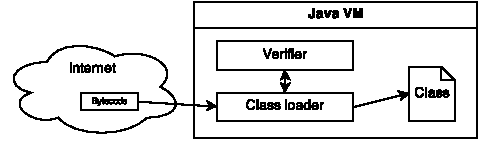
\includegraphics[width=0.8\textwidth]{dia_java_classload.pdf}
	\caption{Class loading in Java}
\end{figure}

Java code is loaded into the virtual machine by a special objects called class loaders. The main task of a class loader is extracting bytecode from some external source and passing it on to the bytecode verifier which determines whether it complies with the required language safety properties. Typically it also selects the desired security policy which will be later enforced upon it, and it is the class loader's task to make sure that the newly loaded code will not replace any existing classes (including itself and other security-critical classes) unless this is explicitly allowed. 

Every Java VM provides a simple "primordial" class loader implemented in native code which bootstraps the framework and immediately hands the process over to its loader. Code with sufficient permissions can then define new, potentially simultaneosly active class loaders and arrange them into hierarchies. Since class loaders are also responsible for resolving classes and methods for the code loaded by them, they can be used to create local namespaces, effectively isolating codebases which should not be allowed to interact.

The last component of the Java sandbox is a reference monitor, called the security manager. Before untrusted code is called, the parent can set a thread-local reference to a \class{SecurityManager} object which implements the security policy that is to be enforced. Should the untrusted code attempt to access system or VM resources during its execution, it must do so through the framework API and these methods always consult the active Security Manager before access is granted.

\subsection{Java Native Interface}

Just like bytecode, shared libraries are loaded by a class loader and reside in its namespace. The method resolver then uses a naming convention defined in the JNI specification to bind a Java method (marked \keyword{native}) with a corresponding function in the native library.

\begin{figure}
	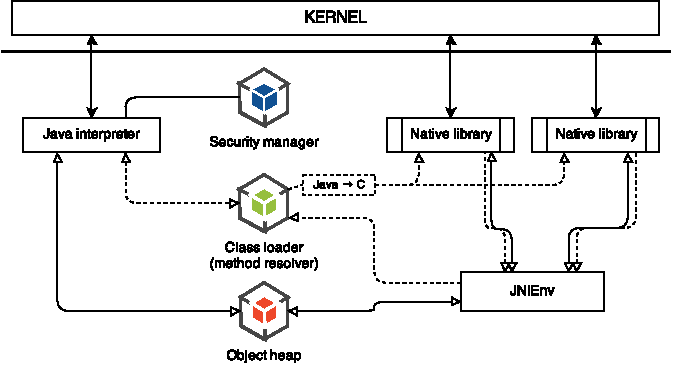
\includegraphics[width=\textwidth]{dia_jni_orig.pdf}
	\caption{Schematic diagram of the core JVM security components with respect to native code. Solid lines represent data flow paths, dashed lines show control flow. [TODO: draw threats in red?]}
	\label{fig:OverviewJNI}
\end{figure}

\begin{figure}[t]
	\lstinputlisting[language=Java,title=HelloJNI.java]{example/HelloJNI.java}
	\lstinputlisting[language=C,title=HelloJNI.c]{example/HelloJNI.c}
	\caption{Example of a method implemented with JNI. \texttt{getMessage} calls \texttt{NewStringUTF} which instantiates a new \texttt{String} object and returns its reference to the caller.}
	\label{listing:HelloJNI}
\end{figure}

Developers are provided with a C/C++ header which contains the definitions of types compatible with the primitive types used in Java, the \texttt{jobject} type to represent object references (typically pointers to the object heap) and the \texttt{JNIEnv} data structure containing functions that provide an API for interfacing with the VM, such as reading/assigning values of object fields, creating new objects, or invoking other managed methods. A pointer to an instance of \texttt{JNIEnv} is passed to the function together with the actual parameters of the corresponding method call. Figure~\ref{fig:OverviewJNI} gives a simplified overview of the architecture, and Figure~\ref{listing:HelloJNI} shows an example of a simple Java class with a \texttt{native} method implemented in C.

However, the Java platform does not provide any means of containing native code. Because it resides in the same virtual address space as the VM, it does have unlimited access to the object heap and can both read and modify any object data on it, including the class loaders. Similarly, native code can perform system calls without the knowledge of the security manager or even modify the state of the virtual machine. Giving a piece of code the permission to load native libraries is therefore equivalent to giving it all the permissions as well as unlimited access to the VM state.

\subsection{Trust and Native Code}

Previous sections have explained the role of the three pillars of Java security: language safety, secure class loading and a reference monitor. To understand how native code fits into this picture, it is essential to understand the relationship between these three components and the assumptions they make.

A Java VM consists mainly of a bytecode interpreter (or a compiler into native code), a minimal class manager with a bytecode verifier, memory management code and a small set of low-level classes implemented in native code which faciliate communication between the VM and the managed code, e.g. to provide reflection. The entire VM codebase must be fully trusted and it must ensure that only safe code will ever be executed.

The framework, on the other hand, is mostly written in Java with a relatively small number of native methods which give managed code access to system calls and only these therefore need to be trusted to not violate language safety. The framework includes classes which abstract over the system resources, provides its own class loader, which selects the appropriate security policy and passes bytecode over to the VM's verifier and loader, and a default implementation of the security manager. All of these Java classes, as well as the native code, are trusted to not compromise the class hierarchy and to always enforce the active security policy.

Since both the developers of the virtual machine and the system administrator have all of the code above under control, trusting it is not a problem. However, when it comes to application code, we immediately see a big discrepancy between programs written purely in Java and those which ship with native libraries. Even if a Java application is not fully trusted, activating the security manager enables the administrator to ensure the safety of its execution. On the other hand, any application with native code must be fully trusted as its safe execution cannot be guaranteed.

\section{Security with Capabilities}

Memory protection and decomposition of software into isolated components are highly desired security properties but contemporary computer systems do not provide the means of achieving them. Most commonly, operating systems provide controlled process isolation with virtual addressing and inter-process communication. This approach, however, suffers from poor scalability due to a high performance penalty imposed by the Translation Look-aside Buffer (TLB) as the number of protection domains and the domain switches between them increases~\cite{watson2012cheri}.

Conversely, capabilities have proven to be a security primitive which allows for fine-grained memory protection and low-overhead software compartmentalization within a single address space. This makes them an ideal tool for applying the principle of least privilege on a very small scale, i.e. running each software component with only the access rights it needs, and that in turn mitigates the consequences of security vulnerabilities which inevitably appear in the code. 

\subsection{Overview of CHERI}

The CHERI extension of the MIPS ISA adds capabilities as a new security primitive that can be utilized by the operating system and other software running on top of it. The result is a hybrid capability architecture which is backwards-compatible with the traditional form of process isolation with virtual address spaces, but simultaneously enables capability-aware software to employ additional security measures within the address space assigned to the running process.

Applications can use CHERI capabilities in many ways. The most elementary use case is treating them as fat pointers~\cite{kwon2013low}, i.e.\ pointers with an upper limit and a set of permissions. This is particularly useful when dealing with pointers to arrays or data structures as the hardware automatically performs zero-overhead runtime bounds checking and thus prevents exploitation of buffer overflow bugs. 

CHERI capabilities can also be sealed, in which case they cannot be used in load/store instructions any more and become pure tokens of authority exchanged between the components. These are the underlying support for the idea of implementing protection domains with \emph{object capabilities}. An object capability consists of a pair of sealed capabilities: 
\begin{inparaenum}[\itshape a\upshape)]
\item a memory region designated to the object with a pointer to an entry function (\emph{code capability}), and
\item a protected argument (\emph{data capability}).
\end{inparaenum}
Each such pair of compatible capabilities can be used by the holder to perform an atomic domain transition with the \insn{CCall} instruction which unseals the two capabilities, sets the limits of accessible memory and jumps to the given function. Object capabilities can therefore be safely passed to an untrusted component (if confined to a non-overlapping memory region) as they only allow access to the internal state of the object via controlled access points. It is easy to see that a similar principle lies at the heart of the object paradigm implemented by Java and other object-oriented languages.

One of the weaknesses typically associated with capabilities is the difficulty of access rights' revocation, e.g.\ after an object is destroyed and its memory region allocated to another. CHERI does not solve this problem entirely and still relies on the software stack to either guarantee virtual space non-reuse or to provide a form of capability garbage collection. It does, however, alleviate the process by enabling capabilities to be marked \emph{ephemeral} and the right to store ephemeral capabilities to be removed from a majority of an object's memory space, hence bounding their potential spread.

\subsection{Protecting Capabilities}

CHERI implements capabilities as 4-word (256-bit) data structures with the following fields:
\begin{description}
	\item[Base \& length] A pointer to the base of the memory region and its length; both 64-bit values.
	\item[Permissions] 31-bit mask which describes the operations that may be performed with the capability.
	\item[Unsealed bit] If this flag is set, the capability can be used in general-purpose capability operations.
	\item[Object type] A 64-bit identificator to ensure that only corresponding code and data capabilities are used together.
\end{description}

Because these are too big to fit into standard registers, CHERI extends the register file with 28 general-purpose and five specialized capability registers, and defines their function in a new ABI convention. Extra caution is required when calling less trusted code because it may not conform to the convention. Specifically, the caller must explicitly clear all unused registers to avoid leaking rights and private data to the callee.

Capabilities must be protected by the hardware yet at the same time it is highly desirable to allow capabilities to be stored together with normal data. To this end, each capability register has a tag which indicates whether it is holding a valid capability or not, and correspondingly the physical memory is required to associate a tag with every fourth word (capabilities in memory must be aligned accordingly). The instructions defined in the extended ISA are then the only ones allowed to set this tag as they are trusted to preserve the security properties, mainly that capability manipulation must never increase rights. Storing into memory with original MIPS instructions always clears the tag of the corresponding capability block. Invoking a capability instruction with an invalid argument traps.

\subsection{Pointer Indirection}

As mentioned earlier, one of the prerequisities of successful compartmentalization of native code is the ability to prevent a component from accessing addresses beyond the region of the virtual address space designated to it. But at the same time, it is important that such containment is seamless in order to retain the ability to run legacy code.

The solution adopted in CHERI is based on pointer indirection, where addresses of all non-capability loads and stores are treated relative to a capability that the active domain carries in register \reg{C0}. Normal pointer to address \texttt{x} then always translates to \texttt{\reg{C0}.base~+~x} and a memory access instruction will trap if \texttt{x~>=~\reg{C0}.length}. 

\reg{C0} initially contains the capability to the entire virtual address space but a less trusted component can be invoked with a capability granting access only to its subset, effectively denying the component access to the rest of the address space without breaking any of its internal pointer arithmetic.

The same principle is applied to instruction fetch from \reg{PC}, only it is indirected through \reg{PCC} which can only be set by the \insn{CCall} instruction.

\subsection{Object Capabilities}

In order to create the pair of capabilities which form an object capability, the object owner first creates an unsealed capability with \emph{seal} and \emph{execute} rights such that the capability's type is a pointer to the entry function relative to the region defined by the base and length, i.e. \texttt{base~+~type~=~\&function} and \texttt{type~<=~length}. Notice that only code which already has the rights to the memory containing the entry function can create this capability. 

The capability is then sealed with the \insn{CSealCode} instruction, becoming the code capability of the object, and is used once more in \insn{CSealData} to seal an arbitrary argument capability. Both components inherit the \emph{object type} field from the unsealed capability.

When a valid object capability pair is passed to the \insn{CCall} instruction, the unsealed code capability becomes the new value of \reg{PCC}, its type is assigned to \reg{PC} and the unsealed data capability is stored in \reg{IDC} (\texttt{=\reg{C27}}). Typically, data capability is the object's memory region and the entry function begins with copying \reg{IDC} to \reg{C0}.

Additionally, \insn{CCall} pushes the old values of \texttt{\reg{PC}~+~4}, \reg{SP}, \reg{PCC} and \reg{IDC} onto a trusted system stack, from which they are restored once the callee invokes \insn{CReturn}.

\subsection{Multithreading}

One of the prevailing limitations of the CHERI prototype is that the trusted thread stack capability is not thread-local and hence it is not safe to perform multiple object calls simultaneously. 

For this reason, the host is currently forced to acquire a lock before it invokes an object capability. Multithreaded access to the sandbox is also not discussed in this dissertation and its implications on the protection mechanisms would require very careful and detailed consideration.

\chapter{Related Work} 

This chapter covers relevant (and typically, recent) research 
which you build upon (or improve upon). There are two complementary 
goals for this chapter: 
\begin{enumerate} 
  \item to show that you know and understand the state of the art; and 
  \item to put your work in context
\end{enumerate} 

Ideally you can tackle both together by providing a critique of
related work, and describing what is insufficient (and how you do
better!)

The related work chapter should usually come either near the front or
near the back of the dissertation. The advantage of the former is that
you get to build the argument for why your work is important before
presenting your solution(s) in later chapters; the advantage of the
latter is that don't have to forward reference to your solution too
much. The correct choice will depend on what you're writing up, and
your own personal preference.

\section{Joe-E}

\section{Dalvik}

sandbox by linux uid

\section{Process-based Isolation}

\section{CCured (SafeJNI)}

\section{SFI (Robusta)}

doesn't support dynamic loading (and by design cannot)

\section{Similar Systems}

\subsection{Joe-E}
\subsection{CORBA}
\subsection{Capsicum}


\chapter{Design and Implementation} 

The proof-of-concept implementation of Qishr is based on JamVM 1.5.4\footnote{http://jamvm.sourceforge.net/}, a highly-portable and compact Java virtual machine, used in combination with the GNU Classpath 0.99 framework\footnote{https://www.gnu.org/software/classpath/}. All changes were contained inside the source code of the virtual machine which means that other frameworks, such as OpenJDK\footnote{http://openjdk.java.net/} or Apache Harmony\footnote{https://harmony.apache.org/}, could be used instead.

\begin{figure}
	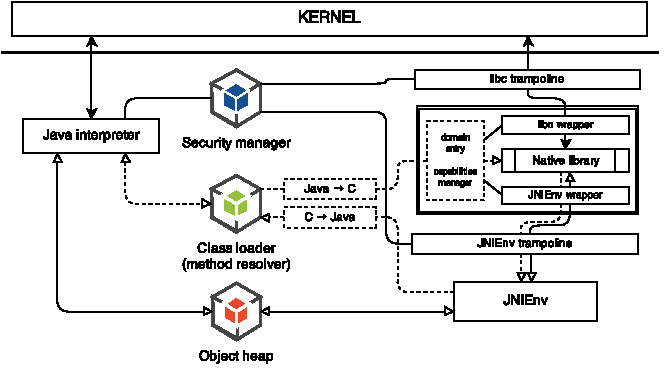
\includegraphics[width=\textwidth]{dia_jni_caps.pdf}
	\caption{Diagram of a Java VM running a native library in a CHERI sandbox. All references are passed across the domain boundary as capabilities.}
	\label{fig:OverviewCheriJNI}
\end{figure}

An overview of the modified design is given in Figure~\ref{fig:OverviewCheriJNI}. As opposed to the the original schematic in Figure~\ref{fig:OverviewJNI}, the native library is now fully contained inside a CHERI sandbox that limits its memory access to a designated region of the virtual address space, thus preventing it from reading or modifying the state of other components. The code is not allowed to perform system calls and similarly cannot directly interact with the VM. Its only option is to invoke a trampoline function inside the host domain which performs the operation on the native code's behalf provided that it is not in conflict with the active security policy.

In order to retain source-level backwards compatibility, the native code can be compiled against \lib{qishr} which provides wrappers for \lib{c} functions and the \texttt{JNIEnv} interface, and also automatically manages the capabilities passed to the sandbox, allowing for seamless integration of legacy code into the sandboxed environment.

\section{Porting Java to CHERI}

Even though the MIPS64 architecture, which CHERI extends, has been around for a while~[REF], processors implementing its instruction set are yet to penetrate the consumer electronics market~[REF]. Software support for this architecture therefore still remains quite rare and its lack proved to be one of the obstacles in the early stages of this project as virtual machines always rely on at least some small amount of assembly code, typically more if optimized for performance. Likewise, the choice of the VM was limited by the fact that the only operating system ported to CHERI to date is FreeBSD, and the only C/C++ compiler capable of producing CHERI code is LLVM/Clang. 

Efforts were initially invested into porting a minimal subset of the Android runtime, ideally the emerging LLVM-based ahead-of-time ART compiler~[FOOT] which will replace the original Dalvik VM~[FOOT] in the future releases of Android. Porting ART to CHERI is especially attractive because it translates Dalvik bytecode (equivalent to Java bytecode) directly to native code optimized for running on resource-restricted platforms much like the CHERI prototype. Being based on LLVM, ART could use the CHERI back-end in order to additionally embrace the security enhancements offered by capabilities while running managed code.

The tight integration of ART (and its numerous dependencies) to a specific platform and toolchain does, however, make porting it to another substrate a very time-consuming task. The obstacles of replacing GCC with LLVM{\slash}Clang in the Android build system have mostly been solved by Linaro~[REF], and ART's pre-existing MIPS32 support and LLVM nature therefore should have made emitting MIPS64/CHERI instructions a straightforward extension. Sadly, fixing its codebase, abundant in Linux-specific code and pointer arithmetic assuming 32-bit pointer length, is far beyond the time frame of this project. With the expected release of 64-bit Android, this path could be revisited.

After a period of experimentation with other Java virtual machines suitable for the embedded environment, the combination of JamVM and GNU Classpath framework was selected for its:
\begin{itemize}
\item complete implementation of the JVM and JNI specifications (versions~5 and 1.4 respectively)
\item strict compliance with POSIX standards
\item minimum amount of platform-specific code
\item overall simplicity of the codebase
\end{itemize}
The price is that JamVM is merely a Java interpreter and thus is unlikely to see a non-negligible performance gain from optimizations which could be achieved with the CHERI ISA, namely hardware bounds checking (a common Java bottleneck~[REF]).

\section{Library Loading}

The process of loading a native library is initiated by calling the \texttt{loadLibrary} method of the \class{System} class. The VM looks for a shared object file of the given name inside lookup folders and attempts to load it with the mechanism approprite for that platform, e.g.\ \lib{dl} on variants of UNIX. When running on CHERI, this mechanism is now replaced with \lib{cheri} -- a library the CHERI SDK provides for managing sandbox instances. 

% \begin{table}
% 	\centering
% 	\begin{tabular}{|c|c|c|}
% 		\hline
% 		\textbf{Start addr}	& \textbf{Purpose} 				& \textbf{Access rights} 	\\
% 		\hline
% 		0x0000				& guard page 					& no access								\\
% 		0x1000				& metadata 						& read only								\\
% 		0x2000				& guard page 					& no access								\\
% 		0x8000				& sandbox image					& read/write 							\\
% 		J + 0x0000			& guard page 					& no access								\\
% 		J + 0x1000			& heap							& read/write							\\
% 		K - 0x1000			& guard page					& no access								\\
% 		K + 0x0000			& stack							& read/write							\\
% 		\hline
% 	\end{tabular}
% 	\caption{Address space layout of a sandbox instance from the point of view of the sandboxed code. \texttt{J} is the first page-aligned address such that the sandbox image fits between \texttt{0x8000} and \texttt{J}. \texttt{K} is equal to the end of the address space minus the size of the stack.}
% 	\label{table:addressSpaceLayout}
% \end{table}

\begin{figure}
	\centering
	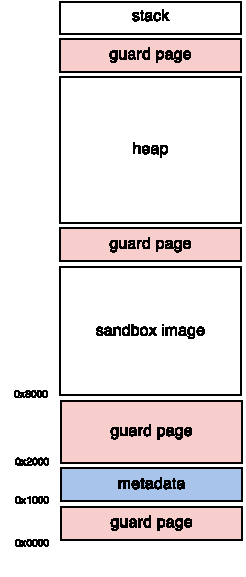
\includegraphics[width=1.0\textwidth]{dia_address_layout.pdf}
	\label{fig:AddressSpaceLayout}
	\caption{Address space layout of a sandbox instance from the point of view of the sandboxed code.}
\end{figure}

\lib{cheri} starts with reserving a memory region for the newly created sandbox, preparing the guest's address space layout as summarized in Figure~\ref{fig:AddressSpaceLayout} and memory mapping the \emph{sandbox image} (library object file) into that region. \label{sec:AddressSpaceLayout}

If successful, it returns two object capabilities. One object represents the sandbox domain, with both the code and data component equal to the designated memory space and the entry point at \texttt{0x8000} as dictated by the CHERI ABI. \label{sec:SystemObject} The other is a system object which the sandbox can use to invoke a method inside the host domain. Its code component is the entire address space of the process, with an entry function inside \lib{cheri} which sets up the capability registers and hands over to a function selected by the host. In order to enable it to identify the domain it was invoked from, the data capability is set to the memory region of the sandbox. The entry function therefore does not set \reg{C0} from the data component but rather from the code capability of the object.

This mechanims is sound and works well for simple examples, but it is still quite undeveloped. The sandbox image must be a statically linked binary stripped off any relocation and symbol information -- so it can be directly mapped to memory -- and have the entry point at a fixed offset. This currently makes it equivalent to Robusta. Conceptually, however, there is no reason why dynamically linked code could not be loaded into the sandbox. As the platform matures, it should therefore become possible to sandbox shared libraries without having to relink or strip them first.

\section{Method Binding}

\subsection{Resolution}

JNI defines a naming convention which encodes the class name, the method name and also its signature into the name of the native symbol that the class loader searches for in the loaded shared libraries. Unfortunately, the fact that CHERI sandbox images currently cannot contain symbol information makes this process more complicated.

For the time being, Qishr uses a simple workaround. When the entry function is invoked with \emph{operation code} \texttt{1} (passed to it in \reg{a0}), the sandbox is expected to extract a function name string from a read-only capability in \reg{C1} and return a non-zero handle if it implements it. Otherwise it should return \texttt{NULL}. The implementation in \lib{qishr} will look for the symbol in a list of function name and pointer pairs pregenerated by the \tool{Ctags} code analyzer\footnote{\url{http://ctags.sourceforge.net/}} and a provided script. The handle is the pointer to the function relative to the base of the inner address space.

\subsection{Invocation}

Operation code \texttt{2} is designated for method invocation, in JNI referred to as \emph{downcall}. The host calls the sandbox object with the handle of the native method it previously acquired in \reg{a1} and the actual parameters in the remaining registers. Primitive arguments are stored in the standard MIPS registers and Java objects as sealed capabilities (\S\ref{sec:MemorySafety}) in the capability registers. Respectively, registers \reg{v0} and \reg{C3} are to be used by the sandbox for the return value.

The number of arguments is currently limited to 6 primitives and 6 objects which is enough for most practical purposes, but the JNI specification allows functions to have up to 255 arguments of any type. A straightforward solution would be to reserve one of the capability registers to pass in a pointer to a buffer containing the arguments which did not fit into registers, much like the MIPS ABI which stores first four arguments in registers and the remainder on the stack.

\lib{qishr}'s entry function sets up the compatibility layers and then simply invokes the function at the given address, which it trusts is valid. 

\subsection{Trap Handling}

At the time of writing, Qishr does not handle situations when the sandboxed code causes a capability-related exception, such as violating the permissions or length. Until very recently, the operating system would handle CHERI traps simply by setting \reg{v0} to negative one, \reg{v1} to the error code and returning to the most recent caller (popping the trusted stack). Because this does not allow the caller to reliably distinguish a successful call from an erroneous one, it has been replaced with sending a UNIX signal to the process but without returning from the domain first.

The sandboxed code could embrace this mechanism to recover from traps and to throw appropriate Java exceptions. It would, however, be necessary to carefully consider the potential effects of allowing the sandbox to handle UNIX signals on the rest of the virtual machine~\cite{989483}.

\section{Interaction with the VM}

The \texttt{JNIEnv} data structure, which each native method receives as its first argument, is the main communication gateway between native code and the managed environment. But because its designers assumed that native code can bypass it any way, it completely lacks any form of protection against misbehaving code. With the native code sandboxed, a \texttt{JNIEnv}-like interface can be the only channel between the sandbox and the VM core, and protecting the core's integrity in the presence of untrusted code becomes worthwhile.

This interface is implemented using the system object capability (\S\ref{sec:SystemObject}) which invokes a \texttt{JNIEnv} trampoline in the system domain. The calling convention again assumes that the first primitive argument is the operation code and the remaining registers are used for the actual parameters of the function. Most of the operations, called \emph{upcalls}, retain the same semantics as their original counterparts, and will simply delegate the call to the corresponding \texttt{JNIEnv} function after the correctness of the arguments is verified. 

Legacy code compiled against \lib{qishr} is provided with a wrapper which translates JNI upcalls to \insn{CCall}s into the host domain.

\subsection{Memory Safety}
\label{sec:MemorySafety}

\begin{figure}[t]
	\begin{lstlisting}[language=C]
jobject point;

// ...

jclass clazz = (*env)->FindClass(env, "java/awt/Point");
if (clazz == NULL) { /* class not found */ }

jfieldID fid = (*env)->GetFieldID(env, clazz, "x", "I");
if (fid == NULL) { /* field not found */ }

(*env)->SetIntField(env, point, fid, 1234);
	\end{lstlisting}
	\caption{JNI code setting the value of a public field.}
	\label{listing:SetFieldValue}
\end{figure}

The main purpose of \texttt{JNIEnv} is enabling the native code to interact with the class hierarchy and the class members in an efficient manner. To this end, native code can request three types of handlers: field identifiers, method identifiers and object references (include class references). Handlers are typically requested by name and JNI returns pointers to the corresponding internal data structures of the VM which makes subsequent upcalls fast. An example of assigning a value to a \keyword{public} field is shown in Figure~\ref{listing:SetFieldValue}. Note that native code is allowed to cache the identifiers but class references are normal object references which can be garbage collected between invocations (\S\ref{sec:LocalAndGlobalRefs}). 

The two main problems with handles are, of course, that they can be dereferenced and forged. For instance, simple arithmetic on an existing object reference suffices to access its private fields as well as compute the handle of the following object on the heap. This can be prevented with sophisticated bookkeeping at the cost of performance, and indeed enterprise JVMs do that, but with CHERI there is another way. 

\subsubsection{Safe Handles}

Because sealed capabilities cannot be tampered with, only passed around, these truly opaque and unforgeable data structures are ideal for representing native handles. The unforgeability is given by the fact that the the \insn{CSealData} instruction copies the object type field from the sealing capability to the result. This field is a 64-bit pointer within the bounds of the sealing capability. Therefore, by setting this field to a location that the sandbox does not have access to, the sandbox will not be able to create the sealing capability and consequently forge the handles. Having multiple sealing capabilities also enables the host to easily distinguish between identify the type of a handle that was passed to it.

Source code written for JNI is built against a header which defines the \texttt{jobject}, \texttt{jfieldID} and \texttt{jmethodID} C/C++ types as \texttt{void*} pointers, but the JNI specification forbids most operations on them. Apart from pointer arithmetic, JNI code should not even test for equality\footnote{\texttt{IsSameObject} upcall should be used instead} as the specification permits two handles to reference one object. The only allowed operation is testing an upcall return value against \texttt{NULL} which in many cases signals an error. Here Qishr employs the fact that Clang for CHERI converts an equality test of a pointer and a capability into a test of its base address. The trampoline will therefore return the \texttt{NULL} capability (an unsealed capability with base and length equal to zero), in which case such test will pass, and a non-\texttt{NULL} sealed capability otherwise. 

Qishr provides its own \texttt{jni.h} header which changes the type definitions of the native handlers. Well-written code should not have any problems building against it as the compiler should automatically modify the layout of all data structures so that capabilities are correctly aligned in memory.

It was also experimented with an alternative approach where \lib{qishr} stored capabilities in its own storage and used pointers into this storage as handles for legacy code. This solution is useful if it is not possible to change the type definitions, either if legacy code is only available in binary form or if the code somehow relies on the original definition. The downside is that the sandbox needs to maintain the storage data structure which necessarily incurs some overhead.

\subsubsection{Access to Class Members}

Safe handles protect against arbitrary access to the address space, but they do not enforce the visibility rules between Java objects, which still allows native code to request handles of class members which it should not have access to. The reason why this is not part of the JNI specification is that native code can easily modify the Java stack and hence change the \emph{execution context}, i.e.\ the class it appears to be a member of. Since the Java stack is now also protected by the sandbox, the execution context information can be trusted and Qishr can enforce this policy at the \texttt{JNIEnv} trampoline. Native code still has the option of using reflection, just like managed code, but the difference is that the use of reflection can be forbidden by the security manager.

\subsubsection{Type Safety}

One other consequence of being forced to fully trust the native code is that, at least in JamVM, upcalls do not verify the types of their arguments which opens the way for type confusion attacks (\S\ref{section:TypeConfusion}). Qishr immediately prevents primitive types from being misinterpreted as object references by the virtue of using capabilities for the latter, and the trampoline calls the type checker for all necessary upcalls, e.g.\ field and array assignments and method invocations.

With all of these mechanisms in place, Qishr can guarantee the memory safety of native code towards Java objects and other internal data structures. Additionally, Qishr can assist as a debugging tool because any violation of these properties will be discovered either by the compiler or at runtime.

\subsection{Memory Management}

Java is known as a language that automatically deallocates unreachable memory, a process famously called \emph{garbage collection} (GC). JNI integrates native code into this scheme by keeping a list of references passed to it and offering it a way of informing the VM that some references are no longer needed. 

But in this scenario, JNI has no assurance that native code will not attempt to use the object reference again later. If the object is garbage collected and the memory allocated to another one, the native code would therefore hold a valid reference to it.

\subsubsection{Object References}
\label{sec:LocalAndGlobalRefs}

JNI distinguishes between three main types of references: local, global and weak global. Every object is by default passed to native code as a \emph{local reference} which remains valid only for the duration of the call. If the native library wishes to retain the reference between invocations of its methods, it can request it to be converted to a \emph{global reference} which will not be garbage collected until explicitly deleted. \emph{Weak global references} also remain valid across invocations, only their existence does not keep the object from being garbage collected at any point and native code must very carefully check their validity before every attempt to use them\footnote{Even if it does, it only shortens the window for an attack by invoking the GC.}. JamVM uses the bottom two bits of the pointer -- objects on heap are aligned to 8 bytes -- to distinguish between these.

Native code needs to remain aware of the number of references it has requested. For instance, if the method creates a large number of small intermediate objects and does not keep their references, they will not be deleted from the list maintained by the VM. For this reason, \texttt{JNIEnv} has several upcalls for signalling that a reference is no longer needed. 

One by one, references can be deleted with \texttt{DeleteLocalRef}, \texttt{DeleteGlobalRef} and \texttt{DeleteGlobalWeakRef}. With local references, there is also an option of creating a new frame on the Java stack with \texttt{PushLocalFrame} and then deleting all the references in it with \texttt{PopLocalFrame}. Unfortunately, JNI specification is very vague about the semantics of these calls and it is unclear what should happen if native code attempts to delete a local reference present in one of the frames deeper in the stack.

\subsubsection{Revoking References}

The implementation in JamVM is therefore very relaxed and code does not even have to be strictly malicious to break the Java stack. Because the correctness of these lists is crucial for safe garbage collection, safety of these upcalls is verified by the trampoline.

\begin{figure}
	\centering
	\texttt{TODO: diagram of the indirection table}
	\caption{Indirection table used for revoking object references}
	\label{fig:IndirectionTable}
\end{figure}

Additionally, Qishr adopts an indirection scheme which enables it to revoke old references. Object references do not point directly to the object heap but rather to an entry in a reference counting hash table unique to each sandbox, depicted in Figure~\ref{fig:IndirectionTable}. Whenever a reference is passed to a sandbox, it is recorded in the JNI frame and its reference count incremented. The counters are decremented whenever a frame is destroyed (Qishr makes sure that all eventually are), or earlier if the sandbox selectively gives up its right to use a reference by deleting it. Any references pointing to a slot with a zero counter are considered invalid. Upcalls invoked with revoked arguments will fail and revoked return values will throw a Java exception.

\subsubsection{Native Garbage Collection}

The design is missing one last key component and that is the ability to reuse entries in the reference table. Right now, an entry of a revoked reference cannot be reallocated because the sandbox could still be holding on to that capability. To this end, Qishr extends the GC to scan the memory region of each sandbox and delete all revoked capabilities. Afterwards, revoked slots can be safely freed and reused.

In general, Java applications cannot make any assumptions about when the garbage collector will be invoked or how it will affect performance. Typically, the VM will run the GC if it fails to allocate memory for a new object on the Java heap. Some VMs, including JamVM, will then lock the entire world until the garbage collection finishes, but Dalvik, for example, is capable of running the GC in a background thread. 

What does not change are the three stages of garbage collection. First, it traverses the Java stack and recursively marks every object it encounters. This is followed by a linear scan of the object heap (\emph{heap sweep}) and deallocation of unmarked objects. If the second step has not freed a fragment large enough for the new object, the GC will attempt again, this time also freeing weak references, and eventually will resort to heap compaction (a very expensive operation). Qishr modifies each one of those stages.

JamVM marking is highly conservative as the GC cannot distinguish native handles from other data. When scanning the native stack of each thread, the marking step will search for values which could be pointers into the object heap. These are marked and recorded as potential \emph{roots}. With Qishr, the C stack of the VM is separate from the C stack of the sandbox, so JamVM will only find its own pointers.

The heap sweep does not need to be changed at all, but Qishr extends it to scrub the memory of sandboxes. This process should be recursive so that all memory reachable from the sandbox is scrubbed, but currently the only memory the sandbox can write into are its own image, stack and heap. The garbage collector does a linear scan of every fourth word, checking if its capability tag is set. Capabilities which 
\begin{inparaenum}[\itshape a\upshape)]
\item are sealed,
\item have type equal to object reference, and
\item their reference count is zero
\end{inparaenum}
will be invalidated by having their first byte overwritten. After the scan, all revoked slots in the reference table are freed.

And lastly, the heap compaction updates the pointers in the indirection table once finished moving the objects. The sealed capabilities do not need to be updated at all as they do not point directly into the object heap.

It should be noted that this makes the garbage collection of JamVM much more precise with respect to native code. In fact, the original marking algorithm can both miss a native handle -- when stored on the native heap -- and interpret random data as one. Respectively, the compaction then either does not update the handle or overwrites a value on the stack. The fact that Qishr indirects all the handles through the reference tables makes updating the pointers available to sandboxes trivial, but the GC can still misinterpret values on the VM's stack. Further research could focus on converting its object pointers to typed capabilities so as to avoid this confusion.

\subsection{Array Operations}

Native code is often employed in otherwise pure-Java applications in order to improve performance while processing large amounts of data, which is why JNI offers several different ways of accessing the elements of Java arrays suitable for different situations.

The most straightforward are upcalls \texttt{Get\-<Type>\-Array\-Region} and \texttt{Set\-<Type>\-Array\-Region} which simply copy the selected range of elements to/from the provided native buffer. The Qishr version of these upcalls requires the pointer to the buffer to be passed as a capability, and the host must very carefully check that the buffer is long enough and that it lies entirely in either the heap or the stack, otherwise it might end up writing into the guard pages. 

\subsubsection{Direct Heap Access}

The second pair of upcalls are \texttt{Get\-<Type>\-Array\-Elements} and \texttt{Release\-<Type>\-Array\-Elements}. The first will return a pointer to a buffer containing the entire array and a boolean which informs the native code whether the buffer is a copy of the elements or whether it is a pointer directly to the object heap (this is called \emph{pinning}). The \texttt{Release} upcall can be called with mode zero (commit changes, free buffer), \texttt{JNI\_COMMIT} (commit changes, keep buffer) or \texttt{JNI\_ABORT} (free buffer, changes will not prevail if data copied). 

JamVM does support pinning which makes array operations with these upcalls very fast. Unfortunately, integrating pinning with the sandbox model is quite complicated. The host has to give the guest a read/write capability to the internal buffer of the Java array because the sandbox cannot access it with a normal pointer. That means later on it must make sure that the \texttt{Release} upcall was invoked~\cite{Kondoh:2008:FBJ:1390630.1390645} and that the sandbox did not keep the capability, while taking into account the possibility of the native code calling other methods, heap compaction being performed, etc. Additionally, changing the return type of the \texttt{Get} upcall to a capability pointer could easily break source-level compatiblity with legacy code. For these reasons, pinning is left to further research and the upcalls are implemented inside the compatiblity layer using the \texttt{Get/Set\-<Type>\-Array\-Region} functions. \lib{qishr} creates a buffer inside the sandbox memory space and then simply copies the array elements between the host and the sandbox as required. Any memory leaks or buffer overflow issues are contained within the sandbox.

\label{ArraysCriticalSection}
JDK 1.3 introduced a third pair of upcalls: \texttt{Get/Release\-<Type>\-Array\-ElementsCritical}. These are very similar to the non-\texttt{Critical} ones, only the native code is not permitted to do anything which could block execution and must treat the scope between these upcalls as a critical section. Under these circumstances, the VM is more likely to grant direct access to the internals of the array even if it normally does not support pinning, e.g.\ by temporarily disabling the garbage collector. These too are currently not supported by Qishr and will resort to copying.

\subsubsection{Direct Buffers}
\label{sec:DirectBuffers}

With the introduction of Java NIO (Non-blocking I/O) in JDK 1.4, JNI was extended with upcalls for interacting with a new set of classes called byte buffers. These, while sharing the same interface, can be backed either by standard Java arrays (\emph{array buffers}) or by a block of memory created by native code (\emph{direct buffers}). The latter are therefore a gateway for Java code into native memory often used in JNI wrappers for native libraries.

Supporting direct buffers in Qishr is also problematic, but in different way to direct array operations. Qishr could translate the address of the native memory block into the host address space, making it available to managed code which runs in the host domain. The issues arise when such buffer is passed to another sandbox which is not allowed to access that part of the memory. At least two potential solutions are at hand, but neither of them without a trade off. Qishr could, for example, create only one sandbox for all native code of a given class loader, but then individual native libraries would stop being protected from one another, or the the \class{DirectByteBuffer} class could be modified to carry a capability pointer, but that would require modifications of legacy code.

For now, Qishr disables the support for direct buffers. Because JVMs are not obliged to provide it, well-written JNI code should always check the type of the buffer before it starts using it, and switch to array operations if necessary. Legacy code used in expertiments therefore worked without any issues.

\subsubsection{Strings}

Similar \texttt{Get/Release} upcalls also exist for operations with Java strings. The difference is that the \class{String} class is supposed to be immutable. JNI code is supposed to honour this property and not change the contents of the underlying \class{char} array even if given direct access to it. Qishr again implements these upcalls with copying and hence guarantees that strings are always immutable.

\subsection{State Consistency}

One of the recurring problems with the Native Interface is that the semantics of upcalls are rather ill-defined, especially in terms of their interference. For instance, \texttt{JNIEnv} provides upcalls for checking whether an exception has been raised (such exception will be thrown after the native method returns), clearing the exception or raising a new one. These enable native code to integrate with the try/catch mechanism of the Java language, but it is unclear which operations should be allowed while there is an exception pending, e.g.\ whether other methods can be called, and similar questions emerge whilst dealing with arrays (\S\ref{ArraysCriticalSection}). 

The lack of a detailed operational model for JNI~\cite{Tan:2010:JNIFormalModel} means that the semantics of these calls are likely to differ between JVMs and native code which runs fine on one could completely break another. Qishr currently does add some \emph{sanity checks} into the trampoline, but a more thorough investigation would be required to guarantee that a sequence of upcalls cannot leave the state of the VM inconsistent. Many previous academic papers address this problem with static analysis~\cite{Kondoh:2008:FBJ:1390630.1390645, Li:2009:FBE:1653662.1653716, Li:2011:JEC:2048066.2048095}.

\section{System Calls}

The CheriBSD operating system currently allows system calls to be invoked only if the \reg{PCC} capability has the \texttt{CHERI\_PERM\_USER0} permission, otherwise a capability exception is raised and the sandbox is killed. Removing this permission from the code capability of the sandbox object thus prevents it from invoking system calls itself and forcing it to use the Qishr trampoline where the active security policy can be enforced.

Code which should run in the sandbox therefore cannot be built against the standard \lib{c}. CHERI SDK provides its own subset (\lib{c\_cheri}) which contains many of the standard C functions that do not involve syscalls, such as operations on strings, \texttt{memcpy} or \texttt{memset}, a sandbox-aware implementation of \texttt{malloc} (reads heap limits from the read-only metadata in the address space; \S\ref{sec:AddressSpaceLayout}) and some glue for setting up the sandbox and invoking the system object. \lib{qishr} then implements the \lib{c} syscall functions (currently 25) as calls into the system domain trampoline, preserving the same semantics.

\subsection{Security Manager}

The active security policy is determined by the active security manager. The VM can either be invoked with a configuration file which the default manager parses, or a \class{Security\-Manager} object can be created programatically and activated before the Java sandbox is entered.

The policy is enforced on a per-thread basis by associating each Java thread with a set of permissions. Before a protected operation is performed, the framework will retrieve the active security manager (also thread-local) with \texttt{System.{\allowbreak}getSecurityManager()} and if it is not \texttt{NULL}, it will call the \texttt{checkPermission} method with the appropriate permission object. Java provides many built-in permissions, but applications can create new ones simply by extending the \class{Permission} class. The \class{Security\-Manager} class defines wrapping methods for the most common checks, such as \texttt{checkRead} for the permission to read a given file or \texttt{checkConnect} for connecting to a given host and port. If the access is not granted, the security manager throws a \texttt{SecurityException}.

Qishr's trampoline integrates native code into this mechanism simply by calling the same methods with JNI upcalls wherever appropriate. As an example, consider the \texttt{open} function. \texttt{open} takes two arguments: a C string with the file path and an integer with bit flags. The bottom two bits determine whether the sandbox requested the file to be opened for reading, writing or both. Accordingly, the trampoline will convert the file path to a Java string, get the object reference of the active security manager and invoke \texttt{checkRead} and/or \texttt{checkWrite} on it. It then checks if an exception has been thrown and if it has, catches it and returns \texttt{-1} with the \texttt{EPERM} error code in accordance with the POSIX specification.

\begin{table}
	\centering
	\scriptsize
	\tt
	\begin{tabular}{|c|l|l|}
		\hline
		\normalfont\bfseries System Call	& \normalfont\bfseries Check Method	& \normalfont\bfseries Condition \\
		\hline
		accept						& checkAccept(String host, int port) 		& \\
		access						& checkRead(String file)				& mode \& R\_OK  \\
		access						& checkWrite(String file)				& mode \& W\_OK \\
		connect						& checkConnect(String host, int port)		& \\
		dlopen						& checkLink(String lib)				& \\
		fopen						& checkRead(String file)				& mode \textnormal{contains} 'r' \\
		fopen						& checkWrite(String file)				& mode \textnormal{contains} 'w' \textnormal{or} 'a' \\
		exit							& checkExit(int status)				& \\
		listen						& checkListen(int port)				& \\
		open							& checkRead(String file)				& flags \textnormal{contain} O\_RDONLY \textnormal{or} O\_RDWR \\
		open							& checkWrite(String file)				& flags \textnormal{contain} O\_WRONLY \textnormal{or} O\_RDWR \\
		rename						& checkWrite(String file)				& \\
		rmdir						& checkDelete(String file)				& \\
		system						& checkExec(String cmd)				& \\
		unlink						& checkDelete(String file)				& \\
		\hline
	\end{tabular}
	\normalfont\normalsize
	\caption{Example mapping of system calls to Java security policy checks.}
	\label{table:SecurityChecks}
\end{table}

Table~\ref{table:SecurityChecks} shows a non-exhaustive list of other system calls and the permission checks they should be mapped to. Only some of these were actually implemented in the proof-of-concept version of Qishr. For production release, all aspects of the syscall functions' semantics would have to be carefully considered and new permissions potentially created for a more fine-grained control.

\subsection{File Descriptors}

The protected system calls are typically ones which ask the kernel to perform an operation on a file (in the UNIX sense of the word). After a file is opened, the process and the kernel refer to it with a \emph{file descriptor}, an integer selected by and registered with the kernel. Qishr, performing system calls on behalf of the sandboxes, needs to keep track of the file descriptors each sandbox is allowed to use at any given point.

Since file descriptors are 16-bit integers, it suffices to create a table capable of storing $2^{16}$ bit flags for each sandbox and then simply set the corresponding bit whenever a file descriptor is created, e.g.\ with \texttt{open} or \texttt{socket}, and clear it as soon as it is closed. In this scheme, a file descriptor value is always available to at most one domain at a time\footnote{With the exception of the standard stream descriptors \texttt{stdin=0}, \texttt{stdout=1} and \texttt{stderr=2} which are always available to all domains.}, and hence a malicious native method will never be able to interfere with files opened by the VM or another sandbox. However, it is important that this analysis is precise or at least conservative. For instance, files opened with the \texttt{O\_CLOEXEC} flag will be closed by the kernel after any system call from the \texttt{exec*} family, which Qishr would not register. Hence it must first clear the permission bit for all the sandboxes before it assigns a newly opened file descriptor to one.

Experiments were also carried out with file descriptors replaced with sealed capabilities, though they currently do not offer any significant advantage. In fact, using them requires a revocation scheme and garbage collection in the same way as with object references, but they also open way for sharing file descriptors between domains. Since Java provides its own abstraction over file descriptors (the \class{FileDescriptor} class), future work could attempt to unify these two approaches.

\chapter{Evaluation} 

A working prototype of Qishr was implemented as an extension to the JamVM embedded Java interpreter, comprising of circa 2,000 lines of C code and 200 lines of MIPS64 assembly. The \lib{qishr} compatibility layer amounted to additional 1,800 lines of C and 100 lines of assembly. Further changes have been made to the build systems of JamVM and GNU Classpath in order to generate binaries compatible with the CHERI sandbox.

Porting took too long?

\section{Trusted Code Base}

\section{Performance}

The additional security measurements inserted into JamVM naturally have an impact on its performance. The overhead imposed by Qishr was measured on a prototype of CHERI, running on an Altera DE4 FPGA development board at 100MHz. 

All experiments were executed with highest priority and Ethernet disabled (current driver keeps polling the device) but the results still suffered from high variation caused by frequent context switches. Time measurements were therefore sorted and the largest 10\% were removed as outliers. 

\subsection{Wrapping Native Libraries}

One of the common use cases for the Java Native Interface is employing either more mature or better optimized third-party native libraries into a Java application. In such situations, JNI servers merely as a wrapper of the native code so it can be invoked from the Java environment.

This scenario was tested on Qishr with a wrapper for \lib{sodium}, a portable cryptographic library aiming to simplify data encryption with clean API and secure default values. A small JNI wrapper was written in 270 lines of C and 150 lines of Java, and compiled both as a shared library and a sandbox image. The native portion of the wrapper invokes \lib{sodium} functions with pointers to buffers provided by the Java side, checks the returned values and raises an exception if there was an error. The Java class queries the native library about the necessary buffer sizes, creates either array buffers or direct buffers (\S\ref{sec:DirectBuffers}) based on user configuration, and exposes a pure Java interface which can be used by other application components to generate RSA key pairs and encrypt/decrypt Java strings. 

The testing program initializes the library, generates two key pairs, encrypts a fixed message with one and decrypts it with the other, timing the duration of each step. The experiment was conducted on an unmodified version of JamVM (once with direct buffers and once with array buffers) and on Qishr (array buffers only), each time with 150 repetitions.

\begin{table}[t]
	\centering
	\footnotesize
	\begin{tabular}{|c|c|c|c|}
		\hline
		\bf Test			& \bf JamVM (direct) & \bf JamVM (array) & \bf Qishr	\\
		\hline
		getPublicKeySize	& $78.92 \pm 5.48$ $\mu$s	& $78.43 \pm 5.19$ $\mu$s	& $228.83 \pm 25.35$ $\mu$s \\
		initIDs			& $2.665 \pm 0.955$ ms		& $2.341 \pm 0.829$ ms		& $4.182 \pm 0.745$ ms \\
		generateKeys		& $2.040 \pm 0.146$ s		& $2.045 \pm 0.079$ s		& $2.044 \pm 0.080$ s \\
		encryptData		& $2.016 \pm 0.030$ s		& $2.020 \pm 0.027$ s		& $2.007 \pm 0.023$ s \\
		decryptData		& $1.999 \pm 0.026$ s 		& $2.017 \pm 0.029$ s 		& $2.005 \pm 0.009$ s \\
		\hline
	\end{tabular}
	\caption{Performance overhead of Qishr.}
	\label{table:OverheadSodium}
\end{table}

\begin{figure}[t]
	\centering
	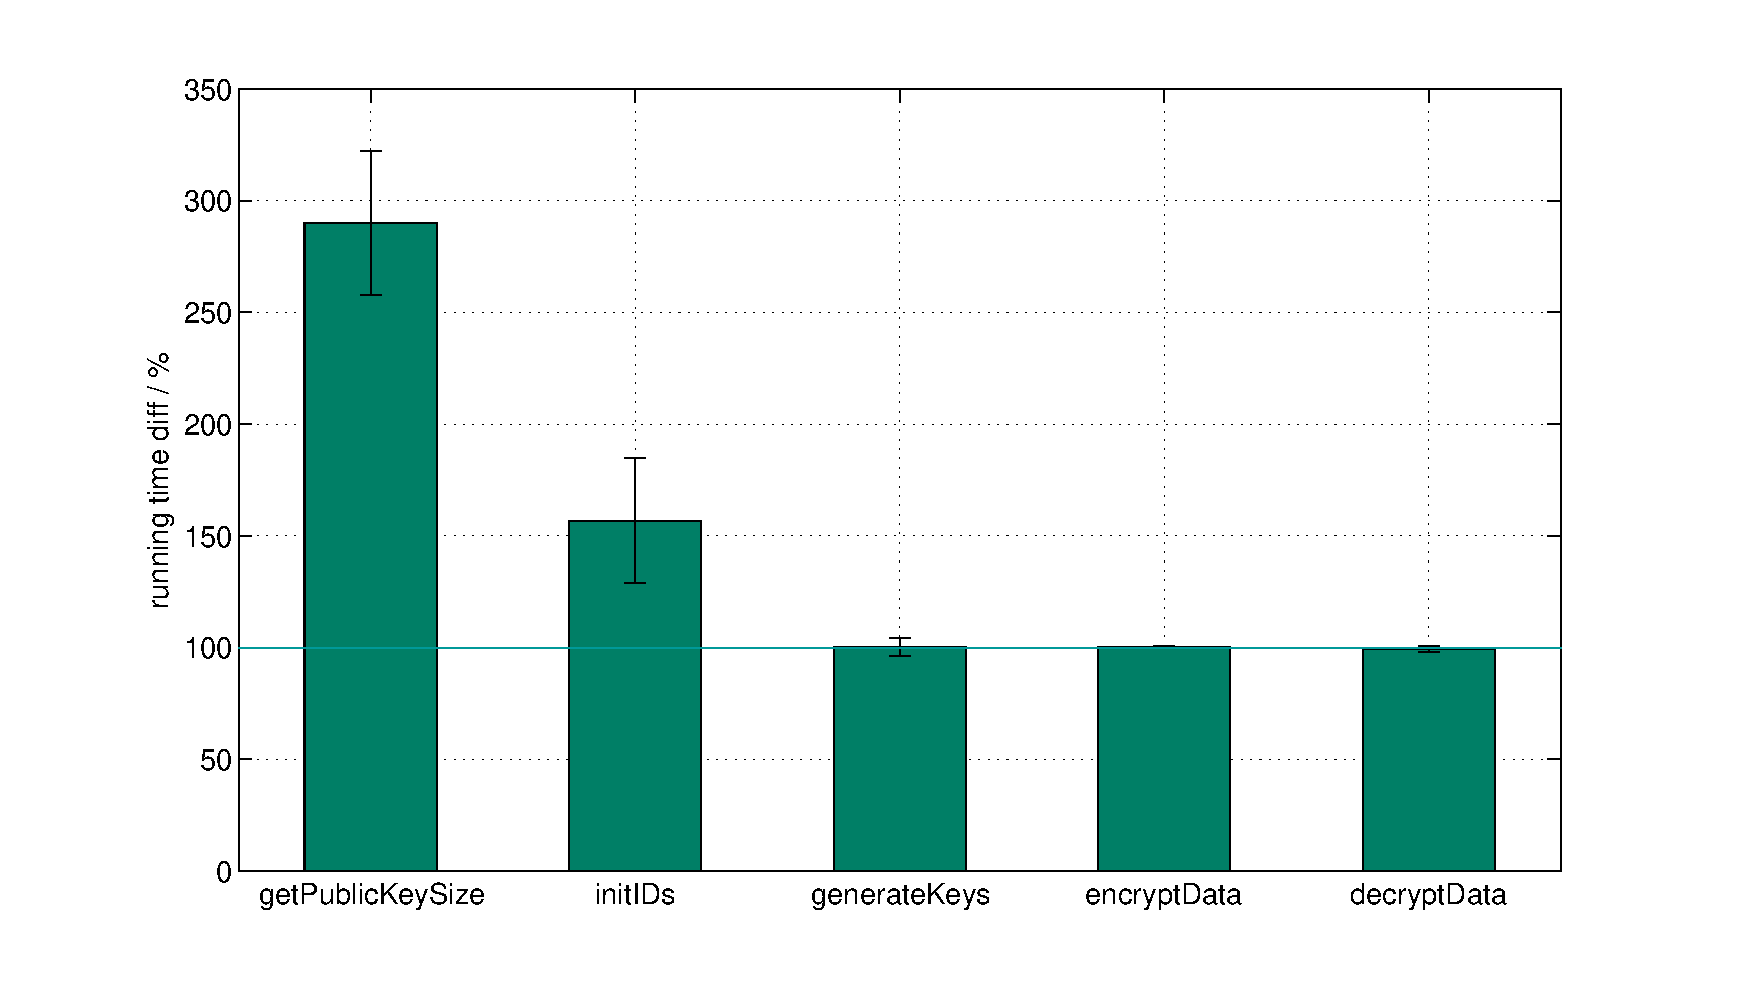
\includegraphics[width=1.1\textwidth]{graph_sodium.eps}
	\caption{Performance overhead of Qishr.}
	\label{fig:OverheadSodium}
\end{figure}

The results are summarized in Table~\ref{table:OverheadSodium} and Figure~\ref{fig:OverheadSodium}. Since JamVM supports pinning (gives direct access to array elements), there was no measurable difference between the two unsandboxed versions. 

\texttt{getPublicKeySize} is a method which only returns a constant defined in the header of \lib{sodium} and it measures the overhead involved in invoking a native method. Regular JNI pops the Java stack and prepares the arguments in accordance with MIPS ABI. With Qishr, this also includes sealing object arguments, switching to the protection domain and setting up \lib{qishr}. That amounts to a small, \emph{roughly} constant $150 \mu$s ($190\%$ more than regular JNI) overhead with each downcall.

\texttt{initIDs} is representative of methods which interact with the VM as its purpose is to request and cache field and method handles for future use. If no errors occur, \texttt{initIDs} requests two class references, one field ID, eight method IDs (11 upcalls in total) and immediately returns. The additional work now also comprises of sealing capabilities, verifying arguments, visibility checks and more domain transitions. However, the overhead, $57\%$, is less significant than in the first case because traversing the class hierarchy involves many string comparisons. 

And this trend only continues as the amount of work done by the native code increases. This is demonstrated by the last three operations which carry out extensive cryptographic computation. They all operate on several small buffers (up to five, each tens of bytes long), each requiring seven upcalls to determine their type and obtain a pointer to the backing buffer. With Qishr that means copying an array in and out of the sandbox. Yet these overheads are so marginal in comparison with the computation itself that the differences between the sandboxed and unsandboxed versions are well within one standard deviation. 

\subsection{Fast Arithmetic}

Performance optimization can be a strong argument for including native code in Java applications but not all operations will benefit from a native implementation. Benchmarks carried out by Kurzyniec et al.~\cite{Kurzyniec01efficientcooperation} show that the enterprise-level JVMs, such as Oracle HotSpot, execute Java bytecode so efficiently that just the JNI invocation overhead itself can far exceed the achieved performance improvement. They conclude that in general, JNI can be used only for heavy computation requiring very little interaction with the VM, such as \lib{sodium} described above. 

\begin{figure}
	\centering
	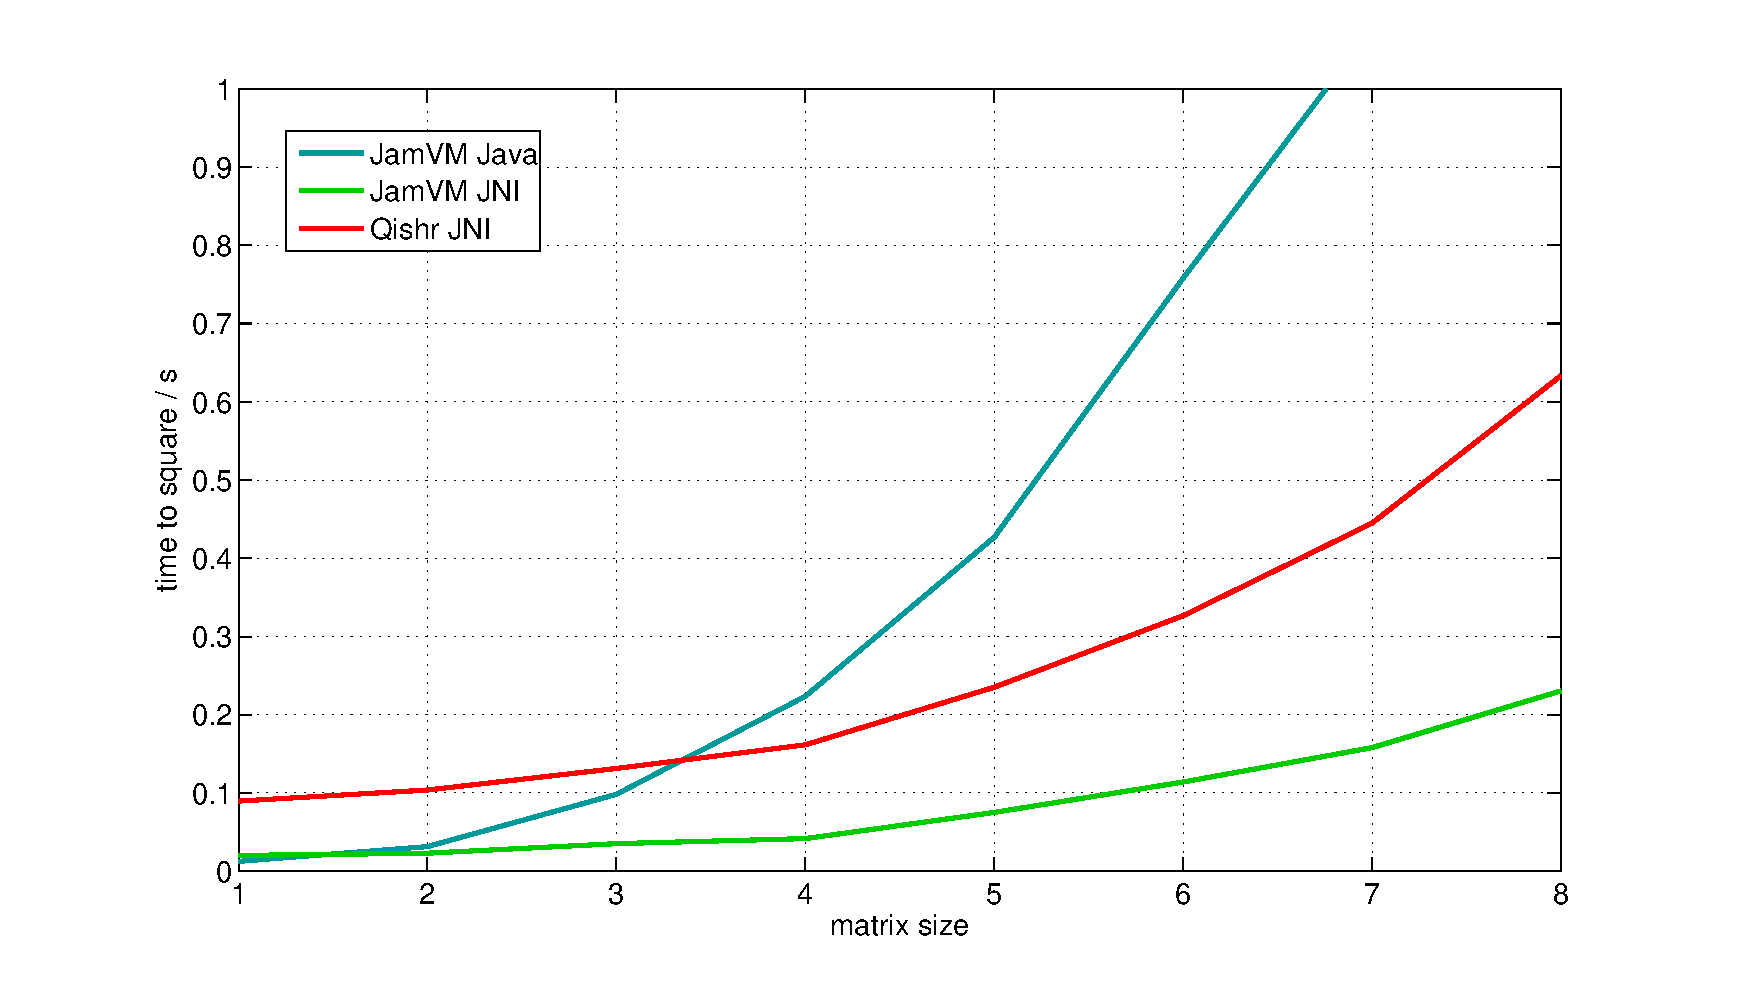
\includegraphics[width=1.1\textwidth]{graph_matrix.eps}
	\caption{Performance overhead of Qishr.}
	\label{fig:OverheadMatrix}
\end{figure}

\begin{figure}
	\centering
	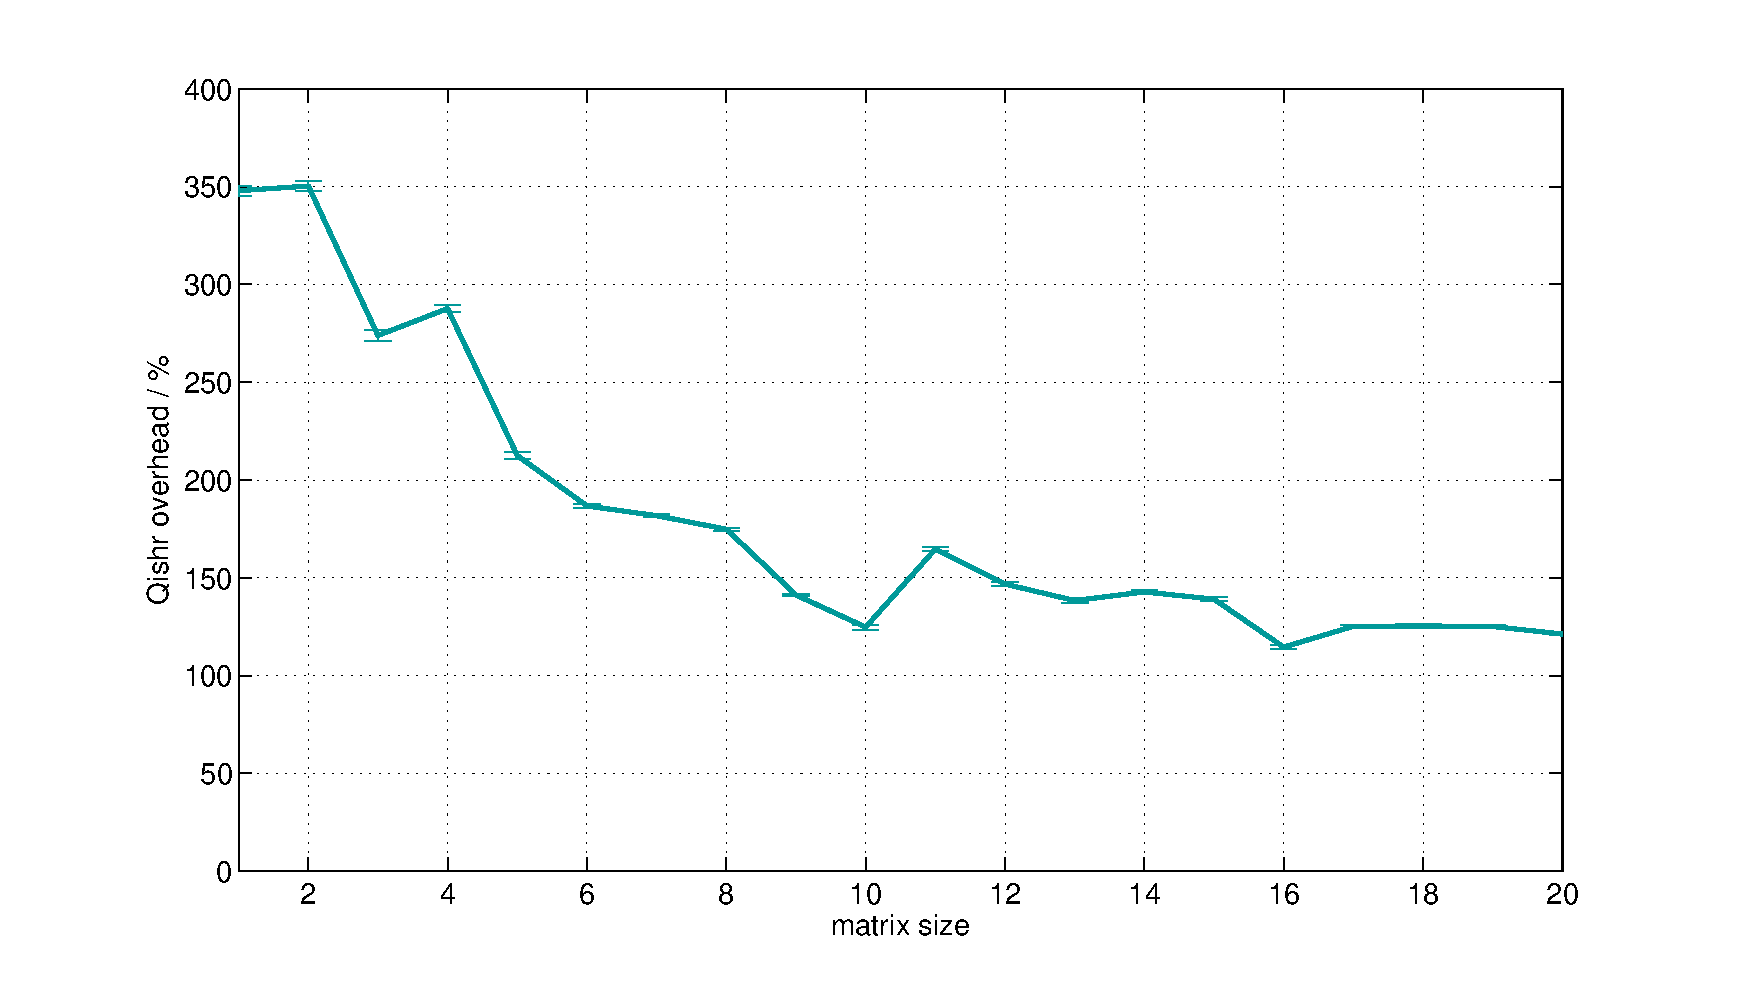
\includegraphics[width=1.2\textwidth]{graph_matrix_subtract.eps}
	\caption{Performance overhead of Qishr.}
	\label{fig:OverheadMatrixSubtract}
\end{figure}


The point when native code becomes faster is necessarily further for Qishr than it is for regular JNI. That, of course, depends on the nature of the operation, but one possible comparison was made by implementing the textbook $O(N^3)$ matrix-squaring algorithm in Java and C. The methods are given two float arrays, one for input and one for output. That way, they only need to access the individual elements of the array and do not, for example, have to allocate new memory. 

Figure~\ref{fig:OverheadMatrix} visualizes the dependence of time taken by each implementation on the size of the matrix. Contrary to the results obtained by Kurzyniec, the overhead of JNI is very small when contrasted with the slow interpreter powering JamVM, and becomes faster as soon as $N=2$. The overhead of Qishr is much higher, outperforming the interpreter by $N = 4$, and this is caused partially by downcalls and upcalls taking longer but mainly by the fact that Qishr keeps copying the matrix in and out of the sandbox.

At the moment, this is Qishr's Achilles heel. Even though the floating-point arithmetic of JamVM is abominably sluggish, the VM at least provides fast access to its arrays. Looking at the plot of the overhead of Qishr over regular JNI in Figure~\ref{fig:OverheadMatrixSubtract} it seems that the difference in their performance tends to somewhere near 110\%, i.e.\ Qishr taking twice as long to finish for sufficiently large matrices. 

Together with the \lib{sodium} test case, these benchmarks show that Qishr does not stand in the way of mostly self-contained native code, but does become a burden once domains start sharing resources. Overcoming the issues with safe direct heap access therefore should be one of the priorities of future work.

\subsection{Cost of Access Control}

\begin{figure}[t]
	\centering
	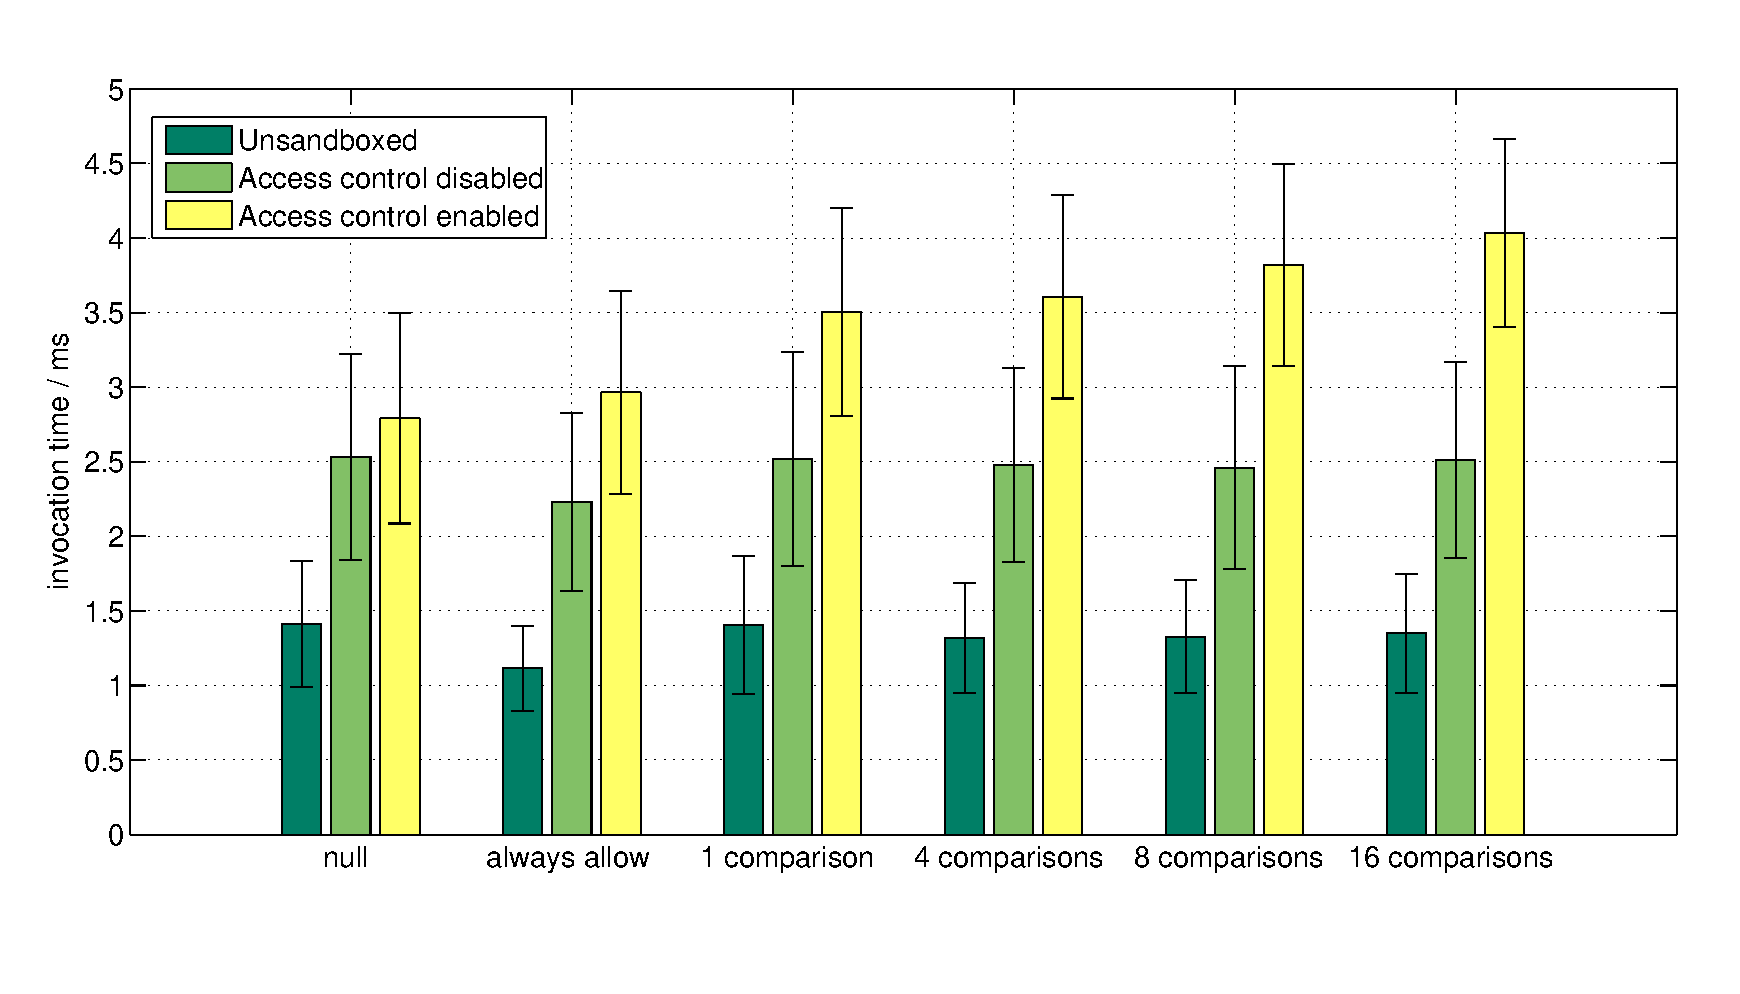
\includegraphics[width=1.1\textwidth]{graph_access.eps}
	\caption{Performance overhead of Qishr.}
	\label{fig:OverheadAccess}
\end{figure}

The other common use for native methods is gaining access to system calls beyond the capacity of the Java framework. Even though the performance does not tend to be an issue in such use cases, the overhead incurred by consulting the Security Manager was measured.

The example application invokes a native method which determines whether a file can be opened in read-only mode with the POSIX \texttt{access} call. Before the method is called, the current Security Manager is set to \emph{null}, one which always allows the call and others which compare the file path against several prefixes. The program was executed in three different modes. The base time required to perform the system call was determined by running it under the unsandboxed JamVM, and the overhead of the downcalls and upcalls with a version of Qishr with access control disabled. And lastly, reenabling access control allows to approximate the overhead of the Security Manager itself. The overall execution times were subtracted and used to produce the breakdown in Figure~\ref{fig:OverheadAccess}.

As expected, the base time and trampoline overhead remain constant, but the time taken to consult the Security Manager rises together with the complexity of the configured security policy. On average, the downcall/upcall management adds $66\%$. Without an active Security Manager, access control adds another $13\%$ which is very reasonable considering several Java methods are invoked in the process. However, if there is a Security Manager, Qishr creates a new Java string with the file path and invokes \texttt{checkRead}, already adding $48\%$ of the base time. 

Access control on Qishr is therefore not cheap, yet still within reasonable bounds. Since the overhead depends on the time taken to run the Security Manager check (implemented in Java), it is very much determined by the complexity of the security policy but also by the speed of the interpreter. Qishr running on top of another VM could hence perform the policy checks much faster.

\subsection{Web Server}

Previous benchmarks each focused on a different aspect of the overhead incurred by Qishr. \emph{NanoHTTPd}\footnote{http://nanohttpd.com/}, a lightweight Java HTTP server, was selected for measurements on a larger, real-life application. Though \emph{NanoHTTPd} does not ship with own native code, its execution inevitably makes extensive use of socket system calls implemented in the native portion of the framework. Running the framework in a sandbox therefore creates the same conditions as if it did.

\begin{table}
	\centering
	\begin{tabular}{|l|c|c|c|}
		\hline
						& \bf JamVM JNI		& \bf Qishr JNI			& \bf Difference \\
		\hline
		static webpage		& $ 9.00 \pm 0.84$ s	& $ 10.50 \pm 0.92$ s 	& $16.61 \pm 10.18$~$\%$ \\
		file server			& $ 101.40 \pm 1.87$ s	& $ 119.28 \pm 2.29$ s 	& $17.64 \pm 2.26$~$\%$ \\
		\hline
	\end{tabular}
	\caption{Overhead measurements for NanoHTTPd.}
	\label{table:OverheadNanoHTTPd}
\end{table}

Two tests were carried out: hosting a small static webpage and downloading 1MB of random data. The client (\emph{curl}\footnote{http://curl.haxx.se/}) was running on another machine connected via Ethernet and first attempts, causing lazy class loading, were thrown away. The results, summarized in Table~\ref{table:OverheadNanoHTTPd}, show a reasonable overhead of roughly $10$-$20\%$ in both cases.

The Java portion of the code runs equally fast on both JVMs and because access control is only applied when \texttt{listen} and \texttt{accept} are being invoked on a socket, it should have almost no impact on the overall performance once the connection is set up. The slowdown is located in the repeated calls to \texttt{write} which sends chunks of data -- passed inside byte buffers -- over the socket, pointing again to array copying as the main source of the overhead.

\chapter{Conclusion} 

Tan et al.\ comprised a list of loopholes in JNI~\cite{Tan06safejava} and experimentally proved that these have the potential to crash at least some JVMs. This section discusses the implications of changes in Qishr on these loopholes.

\begin{description}
\item{\bf Direct Access Through Java References} \\
Object references are truly opaque and sandboxed code is not allowed access outside its memory space, preventing it from retrieving, modifying or corrupting the state of Java objects or the JVM.

\item{\bf Interface Pointers} \\
Individual sandboxes do not share the same instance of \texttt{JNIEnv} and therefore cannot compromise one another by rewriting entries in its function table. Instead, Qishr offers the same functionality with a system-domain trampoline and a \texttt{JNIEnv}-compatible wrapper for the client.

\item{\bf Out-of-bounds Array Access} \\
Array operations are not performed directly on the object heap but rather on their copies inside the framework later copied back by a trampoline function trusted to check the bounds. Any out-of-bounds access is therefore contained within the sandbox and cannot corrupt the data on the Java heap.

\item{\bf Violating Access Control Rules} \\
All field and method ID requests are approved by JamVM's visibility checker. Native code cannot change its execution context since the Java stack is outside the scope of the sandbox.

\item{\bf Manual Memory Management} \\
With regular JNI, native code must inform the JVM once it no longer needs array buffers requested with \texttt{Get\-<Type>\-Array\-Elements} functions (or similar ones), creating a C-like memory management with well known issues such as dangling pointers, multiple releases and memory leaks. Such functions are currently implemented at the compatibility layer using safe operations provided by the trampoline and their incorrect usage can only corrupt the memory of the sandbox. Nevertheless, this safety comes at the price of performance and devising a similar yet controlled interface is needed.

\item{\bf Arguments of Wrong Classes} \\
The trampoline verifies that all object arguments are valid references pointing to objects of the correct type as specified in the signature of the method or field, preventing typing bugs and type confusion attacks. This is possible because the class hierarchy is protected from the sandbox and hence the information can be trusted.

\item{\bf Calling Wrong Methods} \\
Similarly, attempts to access methods, fields and arrays with \texttt{JNIEnv} functions of the wrong type, e.g.\ accessing an \keyword{int} array with \texttt{Get\-Long\-Array\-Elements}, will throw an exception.

\item{\bf Exception Handling} \\
At the moment, Qishr does not address the issues of possible state inconsistency in the presence of a pending exception.

\item{\bf Bypassing the Security Manager} \\
Native code cannot perform potentially dangerous operations on its own. Its only option is calling the system-domain methods defined in the trampoline which consult the active security manager. Untrusted JNI code is therefore fully integrated into the Java Sandbox.

\end{description}

\appendix
\singlespacing

\bibliographystyle{alpha} 
\bibliography{acs-dissertation} 

\end{document}
